\documentclass[tikz,border=6pt]{standalone}
\usepackage{amsmath,amssymb}
\begin{document}
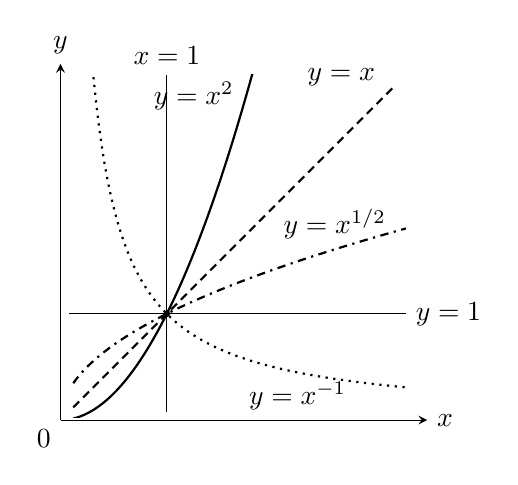
\begin{tikzpicture}[x=1.35cm,y=1.35cm,>=stealth]
  \draw[->,thin] (0,0) -- (3.45,0) node[right] {$x$};
  \draw[->,thin] (0,0) -- (0,3.35) node[above] {$y$};
  \node[below left] at (0,0) {$0$};

  % Images y=x^r in the positive quadrant.
  \begin{scope}
  \clip (0.02,0.02) rectangle (3.32,3.25);
  \draw[thick,domain=0.12:1.82,samples=90] plot (\x,{\x*\x});
  \draw[thick,densely dashed,domain=0.12:3.15,samples=90] plot (\x,\x);
  \draw[thick,dash dot,domain=0.12:3.25,samples=90] plot (\x,{sqrt(\x)});
  \draw[thick,dotted,domain=0.31:3.25,samples=110] plot (\x,{1/\x});
  \end{scope}

  \node[left] at (1.72,3.05) {$y=x^2$};
  \node[above left] at (3.05,3.05) {$y=x$};
  \node[above] at (2.58,1.61) {$y=x^{1/2}$};
  \node[below] at (2.23,0.45) {$y=x^{-1}$};

  \draw[thin] (0.08,1) -- (3.25,1) node[right] {$y=1$};
  \draw[thin] (1,0.08) -- (1,3.25) node[above] {$x=1$};
  \fill (1,1) circle[radius=1.25pt];
\end{tikzpicture}
\end{document}
